\documentclass{article}
\usepackage{cite}
\usepackage{graphicx}
\usepackage{titlesec}
\usepackage{fancyhdr}
\usepackage{lipsum}

\title{test}


\begin{document}

\begin{figure}[h]
  \center
  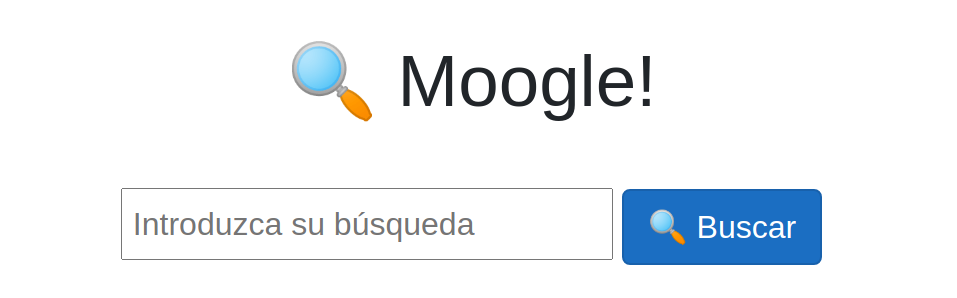
\includegraphics[width=11cm]{moogle.png}
  \caption{Buscador}
  \label{fig:logo}
\end{figure}

Moogle es un buscador de archivos .txt, el cual mediante una consulta debe entregar un grupo de nombres de textos ordenados por relevancia(máximo 3) mostrando una pequeña porción de los mismos donde salgan elementos de la query. Para determinar esta relevancia se utiliza el calculo del TF-IDF, así como también la función coseno.  


\section*{Preprocesamiento}
Al comenzar a ejecutarse el programa los textos son leídos, se les elimina las mayúsculas y los signos de puntuación y es llenado un diccionario(Texts) string, diccionario de string,float donde a cada texto se le hace corresponder sus palabras con la cantidad de veces en las que aparecen. Luego se llena otro diccionario(IDF) de string,float donde se guardan todas las palabras diferentes que aparecen en los documentos y se calcula el idf de cada una. Después se calcula el TF de las palabras en cada texto y estos valores se guardan en el diccionario Text. Teniendo los valores de TF e IDF de cada palabra se procede al cálculo del TF-IDF y estos es almacenan en el diccionario Texts. De esta forma quedan guardados todos los datos necesarios para realizar una consulta y se lanza el buscador.


\section*{Búsqueda}
Cuando el usuario introduce una búsqueda, esta es normalizada de la misma forma que los textos y sus palabras son guardadas en un diccionario(Query) de string,float donde a cada palabra se le corresponde la cantidad de veces en las que aparece en la búsqueda. Luego se calculan los valores de TF de estas palabras y son guardados en el mismo diccionario. Después con el diccionario IDF y el diccionario Query se calcula el TF-IDF de las palabras de la consulta y es almacenado en el diccionario Query. 

Llegado a este punto se procede al calculo de la similitud de la query con los documentos mediante la función coseno. Para esto se utilizan el diccionario Query y el diccionario Texts. Los valores de la relevancia de cada texto son guardados en un array de float. Con este array se cuentan la cantidad de textos relevantes para saber que cantidad de resultados se deben mostrar. 

\section*{Resultados}
Teniendo la cantidad de documentos relevantes se muestran los siguinetes resultados: si no hay ningún texto relevante pues la consulta no coincide con ningún documento y se muestra este mensaje; si hay un documento relevante solo se muestra un resultado con los elementos de este texto; si hay 2 textos pues se muestran los datos de estos textos en funcion con su score y si hay 3 textos o más se muestran los 3 textos más importantes. 

Para realizar todo este proceso de muestra de los resultados se llena un diccionario(TextAndScore) donde a cada ruta del documento se le asocia su valor de relevancia. Luego este diccionario es ordenado de mayor a menor en funcion de los valores de similitud de cada texto. Los elementos de los textos que se muestran son el título y un pequeño snippet (20 palabras a la izquierda y 20 a la derecha de una de las palabras de la consulta).

\section*{Función de ranking}
La correlación se calcula utilizando el coseno del ángulo comprendido entre los vectores documentos(d) y la consulta (q). 

\begin{equation}
sim(d,q) = \frac{\vec{d_j}*\vec{q}}{{|\vec{d_j}|*|\vec{q}|}}
\end{equation}
\begin{equation}
 sim(d,q) = \frac{\sum_{i=1}^{n}w_i,_j*w_i,_q}{\sqrt{\sum_{i=1}^{n}w^2_i,_j}*\sqrt{\sum_{i=1}^{n}w^2_i,_q}}
\end{equation}
$|\vec{d_j}|$ y $|\vec{q}|$ son las normas de los documentos y consulta respectivamente.

\section*{Cálculo del peso en los documentos (TF-IDF)} 
\begin{equation}
  TF-IDF_i,_j = tf_i,_j * idf_i
\end{equation} 

\subsection*{TF}
Sea $freq_i,_j$ la frecuencia del término $t_i$ en el documento $d_j$, entonces, la frecuencia normalizada $f_i,_j$ del término $t_i$ en el documento d_j está dada por: 

\begin{equation}
  tf_i,_j = \frac{freq_i,_j}{max_l freq_l,_j}
\end{equation}

Donde el máximo se calcula sobre todos los términos del documento

\subsection*{IDF}
Sea N la cantidad total de documentos en el sistema y $n_i$ la cantidad de documentos en los que aparece el término $t_i$, la frecuencia de ocurrencia de un término $t_i$ dentro de todos los documentos de la colección $idf_i$ (inverse document frecuency) está dada por:

\begin{equation}
idf_i = \log \frac{N}{n_i}
\end{equation} 

\end{document}